\documentclass[a4paper,12pt,reqno]{amsart}
\usepackage{macros_M66}

\graphicspath{ {images/} }

\begin{document}
%%%%%%%%%%%%%%%%%%%%%%%%%%%%%%%%%%%%%%%%%%%%%%%%%
\hautdepage{TP3: Valeurs singulières, moindres carrés}
%%%%%%%%%%%%%%%%%%%%%%%%%%%%%%%%%%%%%%%%%%%%%%%%%

Vous êtes invité à télécharger le fichier \cmd{tp3\_fonction.sci} qui contient la procédure \sclb{plotimage} nécessaire pour l'exercice 3, ainsi que les fichiers avec des données \cmd{temperatures.dat}, \cmd{lena.dat} et \cmd{george.dat}.

Pour chaque exercice, il va falloir créer un fichier, \cmd{tp3\_exo1.sce}, \dots, \cmd{tp3\_exo3.sce}, comportant les lignes de code correspondant à la résolution de l'exercice. Ces fichiers doivent commencer avec les initialisations habituelles (\sclb{clear},\sclb{clc},\dots).\\[1ex]

% ==================================
\section{Présentation et indications}
% ==================================

% ----------------------------------
\subsection*{Décomposition en valeurs singulières}
% ----------------------------------

Étant donnée une matrice $A\in{\mathcal M}_{m,n}(\R)$ de rang $p\leq \min (m,n)$, la décomposition en valeurs singulières de $A$ est
  $$
    U^tAV = S \quad\text{avec}\quad S = \mbox{diag} (\nu_1, \ldots , \nu_p )
  $$
où les $\{\nu_1 \geq \cdots \geq \nu_p > 0\}$ sont les valeurs singulières non nulles de $A$.

La commande \cmd{Scilab} qui permet d'obtenir cette décomposition pour une matrice \sclb{A} est \sclb{[U,S,V] = svd(A)}. Et pour obtenir juste les valeurs singulières dans un vecteur \sclb{s}$=(\nu_{1},\ldots,\nu_{p})$ il suffit de faire \sclb{s = svd(A)}.

% ----------------------------------
\subsection*{Approximation de rang inférieur}
% ----------------------------------

D'après le théorème de Eckart et Young, la meilleur approximation de rang $k \leq p$, aussi bien en norme $2$ d'opérateur qu'en norme de Frobenius, est donnée par
  $$
    A_{k} = US_{k}V^{t} \quad\text{où}\quad S = \mbox{diag} (\nu_1, \ldots , \nu_k )
  $$

La commande \cmd{Scilab} qui permet d'obtenir cette approximation pour une matrice \sclb{A} est \sclb{[U,S,V] = sva(A,k)}.

% ----------------------------------
\subsection*{Lecture de données à partir d'un fichier}
% ----------------------------------

Étant donné un fichier texte \cmd{nomfichier.dat} contenant $mn$ valeurs, il peut être lu et stocké dans une matrice \sclb{M} de taille $m \times n$ avec la commande \sclb{M = read('nomfichier.dat',m,n);}.


% ==================================
\section{Exercices}
% ==================================

% --------------------------------------------
\begin{exo} (Vérification de résultats du cours)

  \begin{enumerate}
    \item Créer une matrice aléatoire $A$ de taille $30 \times 50$ dont les coefficients suivent la loi uniforme $A_{i,j} \sim \mathcal{U}[-10,10]$.

    \item Représenter sur un graphique la relation entre les valeurs singulières de $A$ et les spectres de $A^{t}A$, de $AA^{t}$ et de
    $
      \left[
        \begin{smallmatrix}
              0 & A \\
          A^{t} & 0
        \end{smallmatrix}
      \right]
    $.

    \item Créer la matrice $B$ qui soit la meilleure approximation de rang $10$ de $A$. Puis calculer, dans une variable \sclb{opt}, l'erreur de cette approximation en norme de Frobenius.

    \item Pour un grand nombre (par exemple $1000$) de matrices aléatoires de rang $10$, si possible pas trop différentes de $B$, calculer et stocker dans un vecteur \sclb{err}, leurs erreurs d'approximation de $A$ en norme de Frobenius.

     \item Vérifier visuellement le théorème de Eckart et Young en représentant sur un même graphique les erreurs stockées dans \sclb{err} et la valeur optimale qui se trouve dans \sclb{opt}.

  \end{enumerate}

\end{exo}


% --------------------------------------------
\begin{exo} (Visualisation des approximations de rang inférieur)

  Les fichiers \cmd{lena.dat} et \cmd{george.dat} contiennent les valeurs matricielles qui représentent les images suivantes:

  \begin{center}
    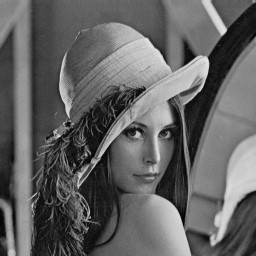
\includegraphics[width=3cm]{lena} \qquad 
\includegraphics[width=3cm]{george}
  \end{center}

  Dans cet exercice, on se propose de visualiser l'approximation de ces images par des matrices de rang inférieur.
  \begin{enumerate}
    \item Stocker les valeurs d'une de ces deux images dans une matrice \sclb{photo} de taille $256 \times 256$. L'affichage de cette photo peut se faire avec la commande \sclb{plotimage(photo)} qui se trouve dans le fichier \cmd{tp3\_fonction.sci}.

    \item Afficher sur 4 graphiques côte-à-côte l'image choisie ainsi que les approximations de rang $5$, $25$ et $75$ de cette même image.
  \end{enumerate}

\end{exo}


% --------------------------------------------
\begin{exo} (Approximation au sens des moindres carrés)

  D'après l'exercice 4 de la feuille de TD3, la résolution au sens des moindres carrés du système $AX=B$ est équivalente à la résolution du système $A^{t}AX=A^{t}B$. Et si le rang de $A$ est égal au nombre de variables (qui est égal au nombre de colonnes de $A$), alors cette solution est unique.

  On se propose dans cet exercice de déterminer le polynôme de degré $2$ qui approxime au mieux, au sens des moindres carrés, l'évolution de la température à Villeneuve d'Ascq pendant un mois.

  \begin{enumerate}
    \item Le fichier \cmd{temperatures.dat} contient les valeurs\footnote{source des données : www.accuweather.com} de la température relevées à midi chaque jour à Villeneuve d’Ascq au mois de janvier 2015. Stocker ces données dans un vecteur colonne \sclb{temp}.

    \item On cherche le polynôme $P \in \mathbb{R}_{2}[X]$ de meilleure approximation au sens des moindres carrés de cette évolution, c'est-à-dire celui qui réalise le minimum de
    $$
      \sum_{i=1}^{30} |T_{i}-P(i)|^2,
    $$
    où les $T_{i}$ sont les températures stockées dans \sclb{temp}.
    Soit \sclb{P} le vecteur colonne à trois coordonnées qui contient les coefficients de $P$.
    Écrire la matrice \sclb{A} du système linéaire \sclb{A*P=temp} qui correspond à $P(i)=T_{i}$ pour $i=1,\ldots,30$.

    \item Résoudre ce système au sens des moindres carrés et stocker les $30$ valeurs approchées de la température dans une variable \sclb{apptemp}.\\
    \textit{Rappel: Comme vous l'avez appris au \textup{S5}, pour résoudre un système de la forme $SX=Y$ il ne faut surtout pas inverser $S$ pour trouver $X$ sous la forme $X = S^{-1}Y$.}

    \item Afficher sur un même graphique les valeurs relevées et les valeurs approchées de la température pendant ce mois.
  \end{enumerate}

\end{exo}

%%%%%%%%%%%%%%%%%%%%%%%%%%%%%%%%%%%%%%%%%%%%%%%%%
\end{document}
